\documentclass[aspectratio=169]{../latex_main/tntbeamer}  % you can pass all options of the beamer class, e.g., 'handout' or 'aspectratio=43'
\usepackage{dsfont}
\usepackage{bm}
\usepackage[english]{babel}
\usepackage[T1]{fontenc}
%\usepackage[utf8]{inputenc}
\usepackage{graphicx}
\graphicspath{ {./figures/} }
\usepackage{algorithm}
\usepackage[ruled,vlined,algo2e,linesnumbered]{algorithm2e}
\usepackage{hyperref}
\usepackage{booktabs}
\usepackage{mathtools}

\usepackage{amsmath,amssymb}

\DeclareMathOperator*{\argmax}{arg\,max}
\DeclareMathOperator*{\argmin}{arg\,min}

\usepackage{amsbsy}
\newcommand{\vect}[1]{\bm{#1}}
%\newcommand{\vect}[1]{\boldsymbol{#1}}

\usepackage{pgfplots}
\pgfplotsset{compat=1.16}
\usepackage{tikz}
\usetikzlibrary{trees} 
\usetikzlibrary{shapes.geometric}
\usetikzlibrary{positioning,shapes,shadows,arrows,calc,mindmap}
\usetikzlibrary{positioning,fadings,through}
\usetikzlibrary{decorations.pathreplacing}
\usetikzlibrary{intersections}
\pgfdeclarelayer{background}
\pgfdeclarelayer{foreground}
\pgfsetlayers{background,main,foreground}
\tikzstyle{activity}=[rectangle, draw=black, rounded corners, text centered, text width=8em]
\tikzstyle{data}=[rectangle, draw=black, text centered, text width=8em]
\tikzstyle{myarrow}=[->, thick, draw=black]

% Define the layers to draw the diagram
\pgfdeclarelayer{background}
\pgfdeclarelayer{foreground}
\pgfsetlayers{background,main,foreground}

% Requires XeLaTeX or LuaLaTeX
%\usepackage{unicode-math}

\usepackage{fontspec}
%\setsansfont{Arial}
\setsansfont{RotisSansSerifStd}[ 
Path=../latex_main/fonts/,
Extension = .otf,
UprightFont = *-Regular,  % or *-Light
BoldFont = *-ExtraBold,  % or *-Bold
ItalicFont = *-Italic
]
\setmonofont{Cascadia Mono}[
Scale=0.8
]

% scale factor adapted; mathrm font added (Benjamin Spitschan @TNT, 2021-06-01)
%\setmathfont[Scale=1.05]{Libertinus Math}
%\setmathrm[Scale=1.05]{Libertinus Math}

% other available math fonts are (not exhaustive)
% Latin Modern Math
% XITS Math
% Libertinus Math
% Asana Math
% Fira Math
% TeX Gyre Pagella Math
% TeX Gyre Bonum Math
% TeX Gyre Schola Math
% TeX Gyre Termes Math

% Literature References
\newcommand{\lit}[2]{\href{#2}{\footnotesize\color{black!60}[#1]}}

%%% Beamer Customization
%----------------------------------------------------------------------
% (Don't) Show sections in frame header. Options: 'sections', 'sections light', empty
\setbeamertemplate{headline}{empty}

% Add header logo for normal frames
\setheaderimage{
	% 
\includegraphics[height=\logoheight]{figures/TNT_darkv4.pdf}
	
\includegraphics[height=\logoheight]{../latex_main/figures/luh_logo_rgb_0_80_155.pdf}
	% 
\includegraphics[height=\logoheight]{figures/logo_tntluh.pdf}
}

% Header logo for title page
\settitleheaderimage{
	% 
\includegraphics[height=\logoheight]{figures/TNT_darkv4.pdf}
	
\includegraphics[height=\logoheight]{../latex_main/figures/luh_logo_rgb_0_80_155.pdf}
	% 
\includegraphics[height=\logoheight]{figures/logo_tntluh.pdf}
}

% Title page: tntdefault 
\setbeamertemplate{title page}[tntdefault]  % or luhstyle
% Add optional title image here
%\addtitlepageimagedefault{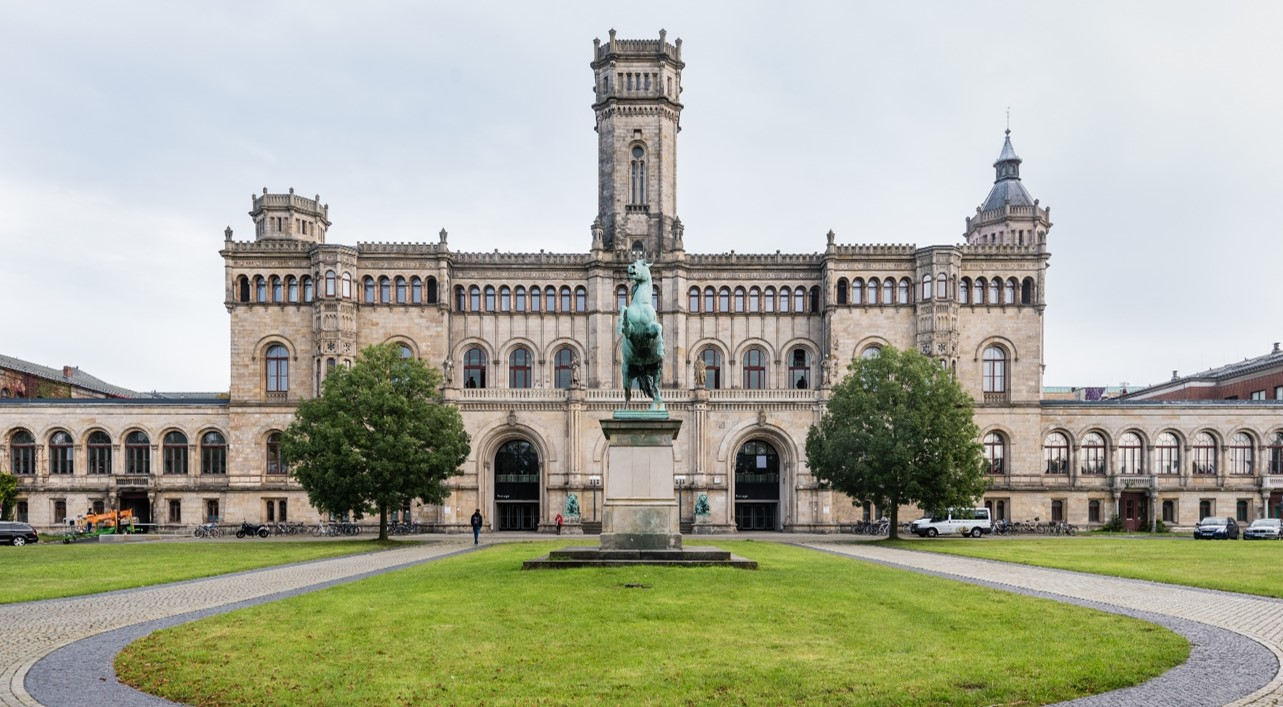
\includegraphics[width=0.65\textwidth]{figures/luh_default_presentation_title_image.jpg}}

% Title page: luhstyle
% \setbeamertemplate{title page}[luhstyle]
% % Add optional title image here
% \addtitlepageimage{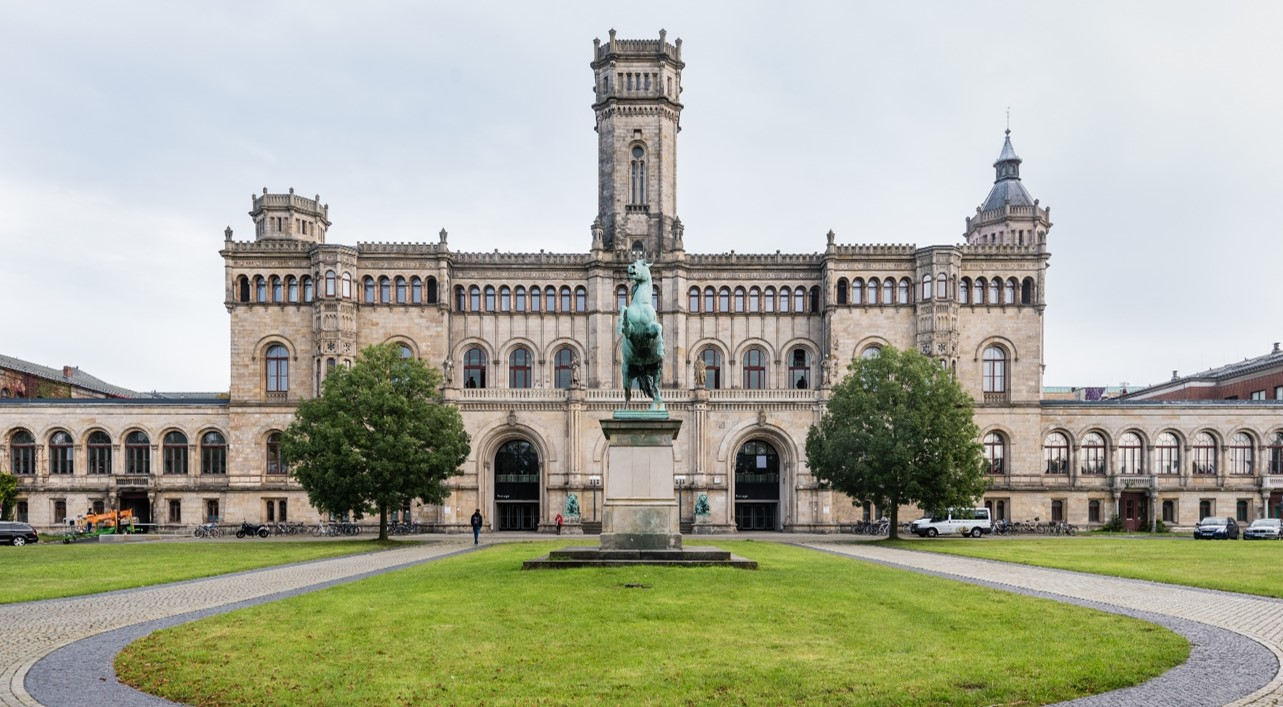
\includegraphics[width=0.75\textwidth]{figures/luh_default_presentation_title_image.jpg}}

\author[Abedjan \& Lindauer]{Ziawasch Abedjan \& Marius Lindauer\\[1em]
	
\includegraphics[height=\logoheight]{../latex_main/figures/luh_logo_rgb_0_80_155.pdf}\qquad
	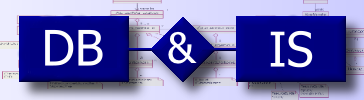
\includegraphics[height=\logoheight]{../latex_main/figures/DBIS_Kurzlogo.png}\qquad

\includegraphics[height=\logoheight]{../latex_main/figures/TNT_darkv4}\qquad

\includegraphics[height=\logoheight]{../latex_main/figures/L3S.jpg}	}
\date{Summer Term 2022; \hspace{0.5em} {
\includegraphics[height=1.5em]{../latex_main/figures/Cc-by-nc-sa_icon.svg.png}}; based on \href{https://ds100.org/fa21/}{[DS100]}
}


%%% Custom Packages
%----------------------------------------------------------------------
% Create dummy content
\usepackage{blindtext}

% Adds a frame with the current page layout. Just call \layout inside of a frame.
\usepackage{layout}


%%% Macros
%\renewcommand{\vec}[1]{\mathbf{#1}}
% \usepackage{bm}
%\let\vecb\bm

\title[Introduction]{DS: Inference for Modeling}
\subtitle{Bootstrapping}

\graphicspath{ {./figure/} }
%\institute{}


\begin{document}
	
	\maketitle
	\begin{frame}{Note}
	    \begin{itemize}
	        \item This section should be review from Data 8.
	        \item The Data 8 textbook does a fantastic job of teaching bootstrapping if you’ve never seen it before.
	    \end{itemize}
	\end{frame}
	
	\begin{frame}{Bootstrap resampling}
	    \begin{itemize}
	        \item To determine the properties (e.g. variance) of the sampling distribution of an estimator, we’d need to have access to the population.
	        \begin{itemize}
	            \item We would have to consider all possible samples, and compute an estimate for each sample.
	        \end{itemize}
	        \item But we don’t, we only have one random sample from the population.
	    \end{itemize}
	    \bigskip
	    Idea: Treat our random sample as a “population”, and resample from it.
	    \begin{itemize}
	        \item Intuition: a random sample resembles the population, so a random resample resembles a random sample.
	    \end{itemize}
	\end{frame}
	
	
	\begin{frame}{Bootstrap resampling}
	    Bootstrap resampling is a technique for estimating the sampling distribution of an estimator.
	    \begin{figure}
	        \centering
	        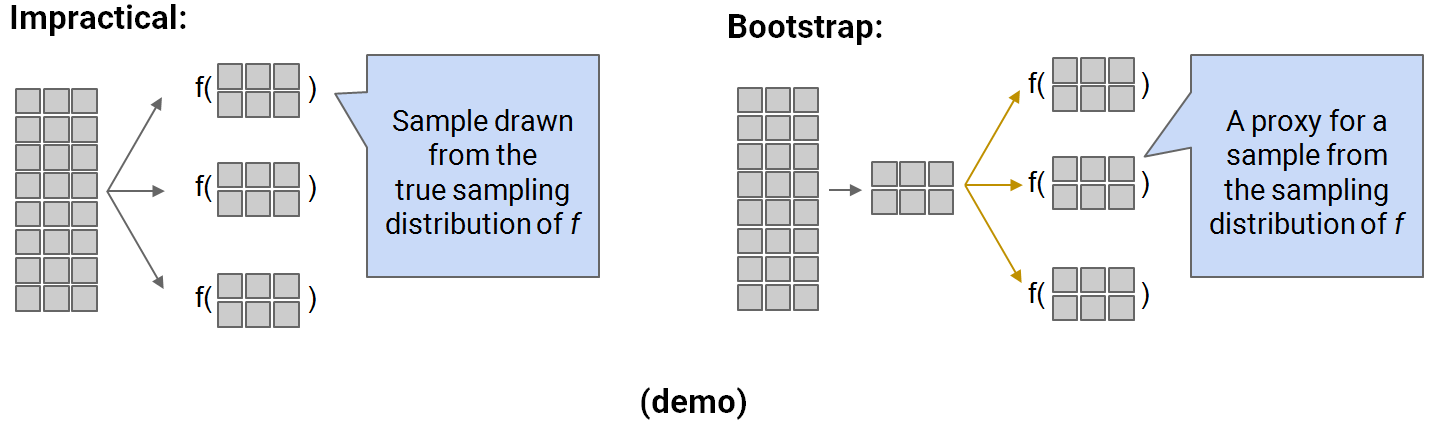
\includegraphics[scale=.4]{Bild4}
	    \end{figure}
	\end{frame}
	
	
	\begin{frame}{Bootstrapping pseudocode}
	    collect random sample of size n (called the bootstrap population)\\
        initiate list of estimates\\
        repeat 10,000 times:\\
        \hspace{2cm} resample with replacement n times from bootstrap population\\
        \hspace{1cm} apply estimator f to resample\\
        \hspace{1cm} store in list\\
        list of estimates is the bootstrapped sampling distribution of f\\
        \hfill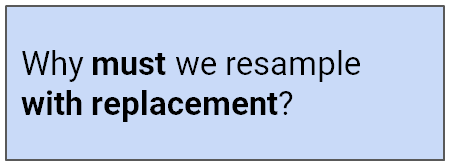
\includegraphics[scale=.5]{Bild5}


	\end{frame}
	
	\begin{frame}{Bootstrap discussion}
	    \begin{itemize}
	        \item The bootstrapped sampling distribution of an estimator does not exactly match the sampling distribution of that estimator.
	        \begin{itemize}
	            \item The center and spread are both wrong (but often close).
	        \end{itemize}
	        \item The center of the bootstrapped distribution is the estimator applied to our original sample.
	        \begin{itemize}
	            \item We have no way of recovering the estimator’s true expected value.
	        \end{itemize}
	        \item The variance of the bootstrapped distribution is often close to the true variance of the estimator.
	        \item The quality of our bootstrapped distribution depends on the quality of our original sample.
	        \begin{itemize}
	            \item If our original sample was not representative of the population, bootstrap is next to useless.
	        \end{itemize}
	    \end{itemize}
	\end{frame}
	
	
	\begin{frame}{.}
	    \begin{figure}
	        \centering
	        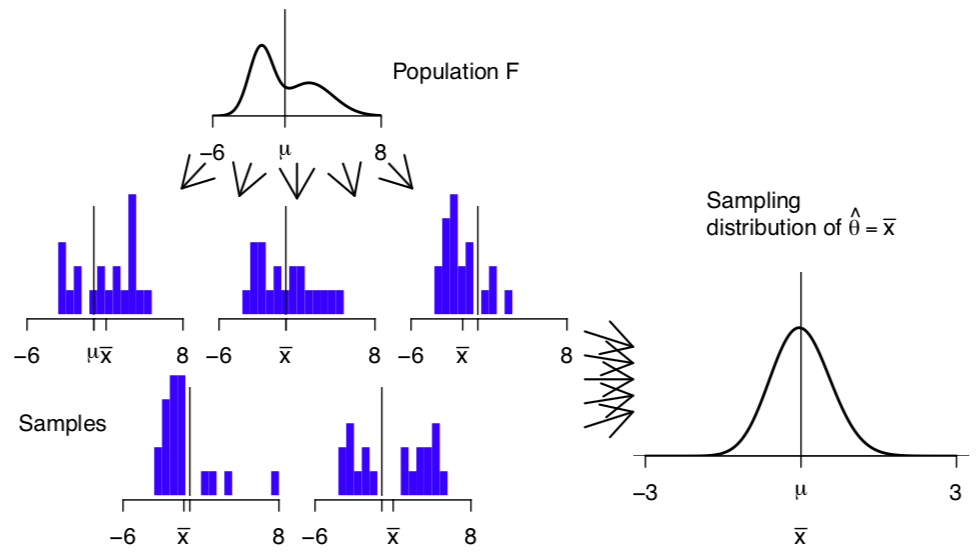
\includegraphics[scale=.45]{Bild6}
	    \end{figure}
	\end{frame}
	
	
	\begin{frame}{.}
	    \begin{figure}
	        \centering
	        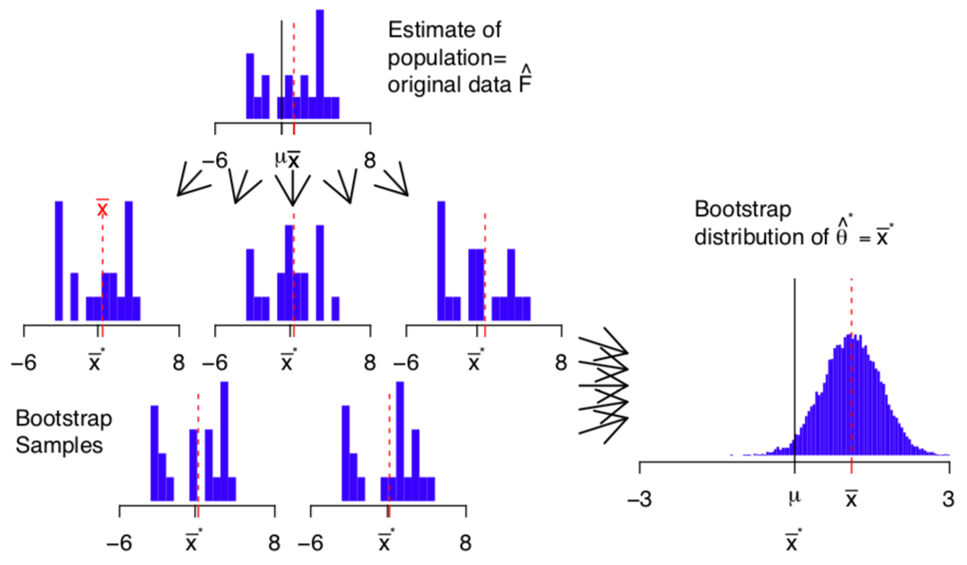
\includegraphics[scale=.45]{Bild7}
	    \end{figure}
	\end{frame}
\end{document}